\documentclass{beamer}

% \usepackage{beamerthemesplit} // Activate for custom appearance
\usepackage{color}
\title{Cryo Microwave Status}
\author{Ana Malag\'on}
\date{\today}

\begin{document}

\frame{\titlepage}

%\section[Outline]{}
%\frame{\tableofcontents}

%\section{Introduction}
%\subsection{Overview of the Beamer Class}
%\frame
%{
%  \frametitle{Features of the Beamer Class}
%
%  \begin{itemize}
%  \item<1-> Normal LaTeX class.
%  \item<2-> Easy overlays.
%  \item<3-> No external programs needed.      
%  \end{itemize}
%}
\begin{frame}
\begin{columns}
\column{0.8\textwidth}
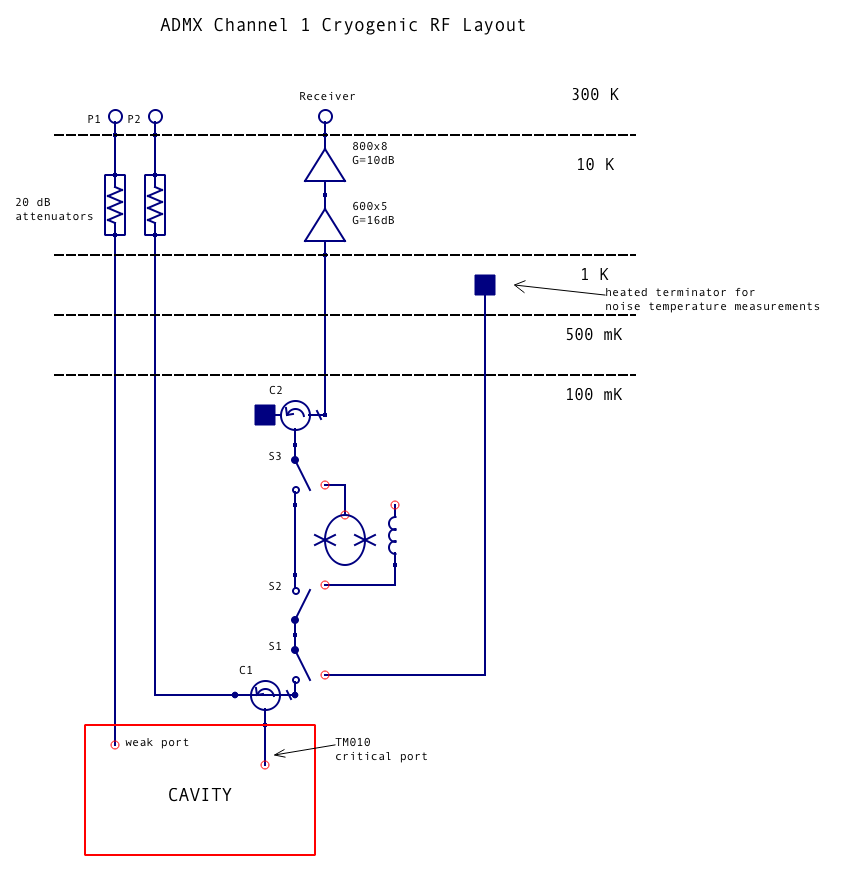
\includegraphics[width=\textwidth]{export_cryo_layout_msa_text}
\column{0.3\textwidth}
\begin{itemize}
\item {\tiny Quinstar Circulators: \\ UTE1255KCS}
\item {\tiny MSA: LFF-12A \\ $T_{MSA}$ @ 100mK = ? \\ Gain = 20 dB}
\item {\tiny HEMTs: \\ $T_{600-5} = 2$ K \\ $T_{800-8} = 10$ K}
\end{itemize}
\end{columns}
%\label{frequency}
%\hyperlink{frequency}{http://admxdatastore.npl.washington.edu/mediawiki/images/2/20/MSA_update_sept2014_Wagner.pdf}
\end{frame}

\begin{frame}
\begin{columns}
\column{0.6\textwidth}
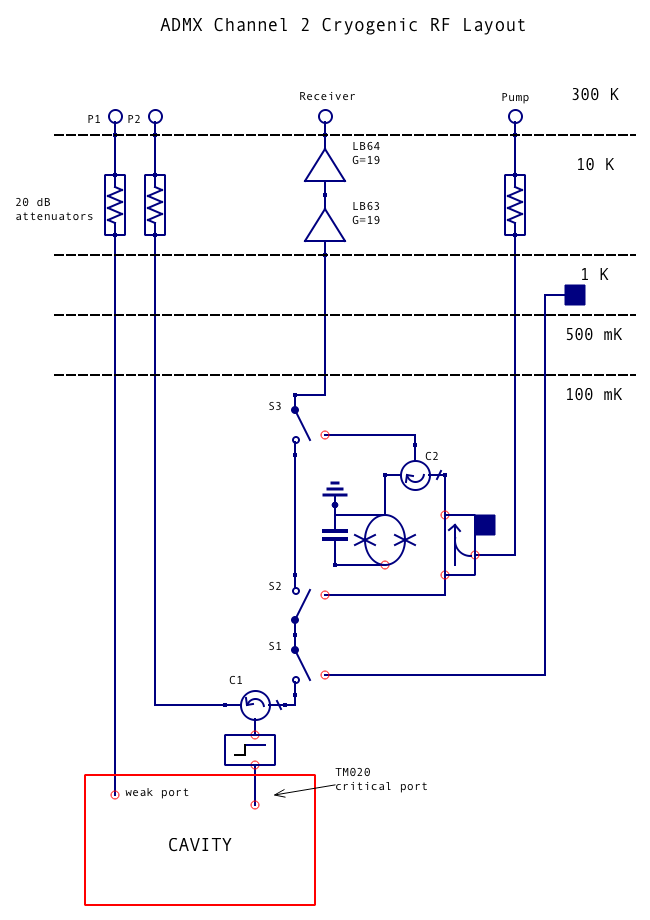
\includegraphics[width=\textwidth]{export_cryo_layout_jpa_text}
\column{0.4\textwidth}
\begin{itemize}
\item {\tiny Quinstar Circulators: \\ LTG0102KCS}
\item {\tiny JPA: \\ $T_{JPA}$ @ 100 mK = ? \\ Gain = 21 dB}
\item {\tiny HEMTs: \\ $T_{LB63} = 6$ K \\ $T_{LB64} = 6$ K}
\end{itemize}
\end{columns}
\end{frame}

\begin{frame}
\begin{columns}
\column{0.6\textwidth}
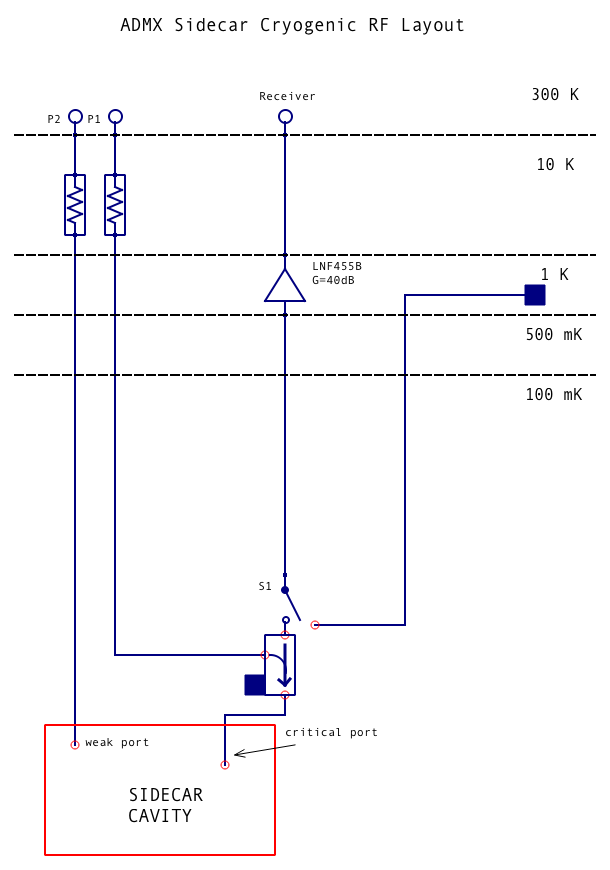
\includegraphics[width=\textwidth]{export_cryo_layout_sidecar}
\column{0.4\textwidth}
\begin{itemize}
\item{\tiny Directional Coupler: PE220120 \\ 20dB coupling}
\item {\tiny HEMT: \\ $T_{LNF455B} = 4$ K}
\item {\tiny $^*$Raditek Circulator: \\ SN102}
\item {\tiny $^*$JPA: \\ $T_{JPA}$ @ 100 mK = ? \\ Gain = ?}
\end{itemize}
{\tiny $^*$ to be put in for second iteration.}
\end{columns}
\end{frame}

\begin{frame}

\begin{columns}
\column{0.3\textwidth}
\centering
{\color{blue} 2014 Squidadel}
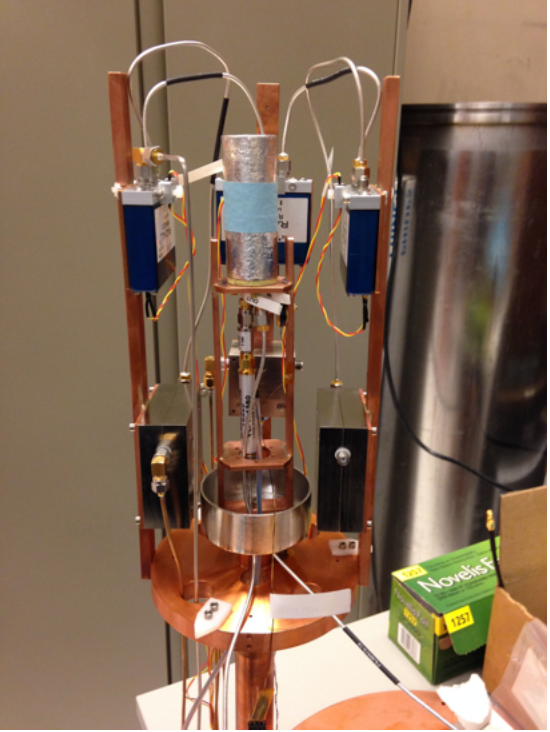
\includegraphics[width=1.1\textwidth]{old_squidadel}
\column{0.3\textwidth}
{\color{blue} add 4 more switches... $\rightarrow$}
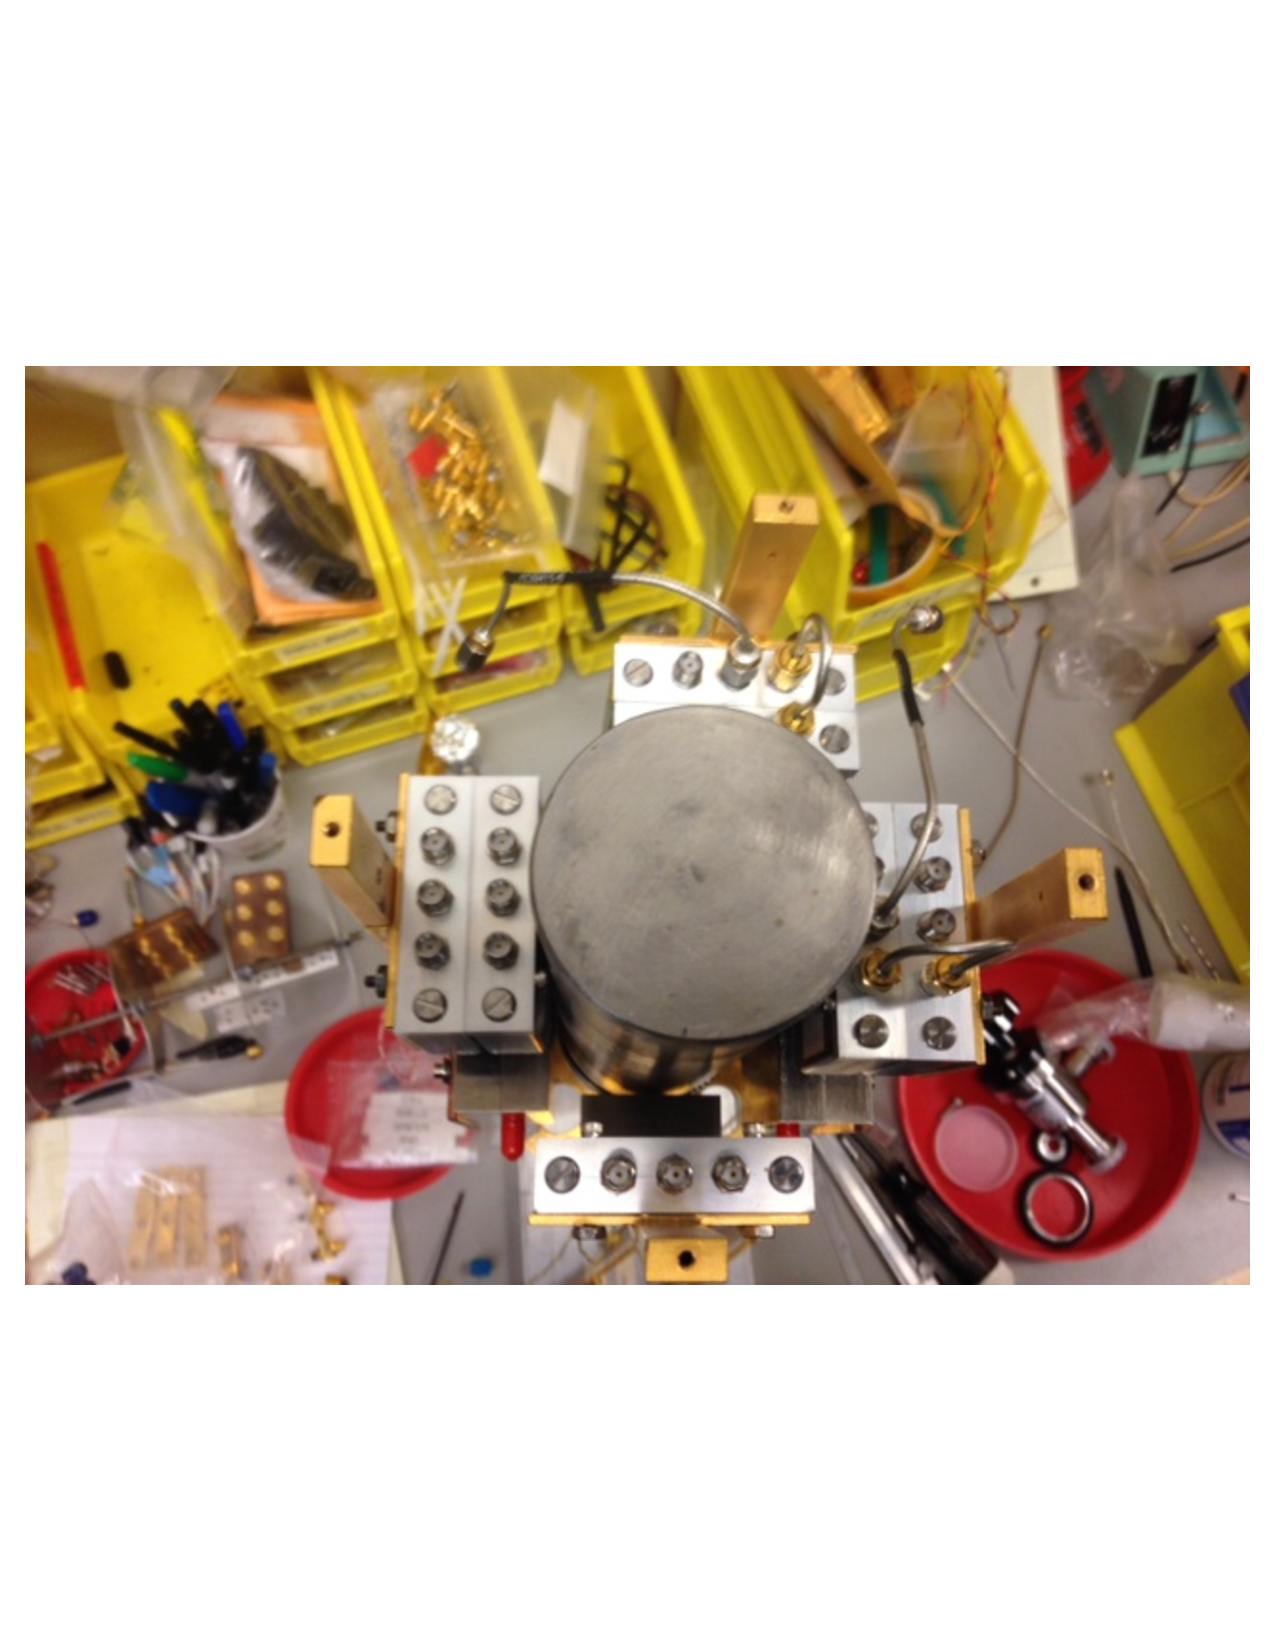
\includegraphics[width=1.1\textwidth]{top_view_squidadel}
\column{0.3\textwidth}
\centering
{\color{blue} 2015 Squidadel}
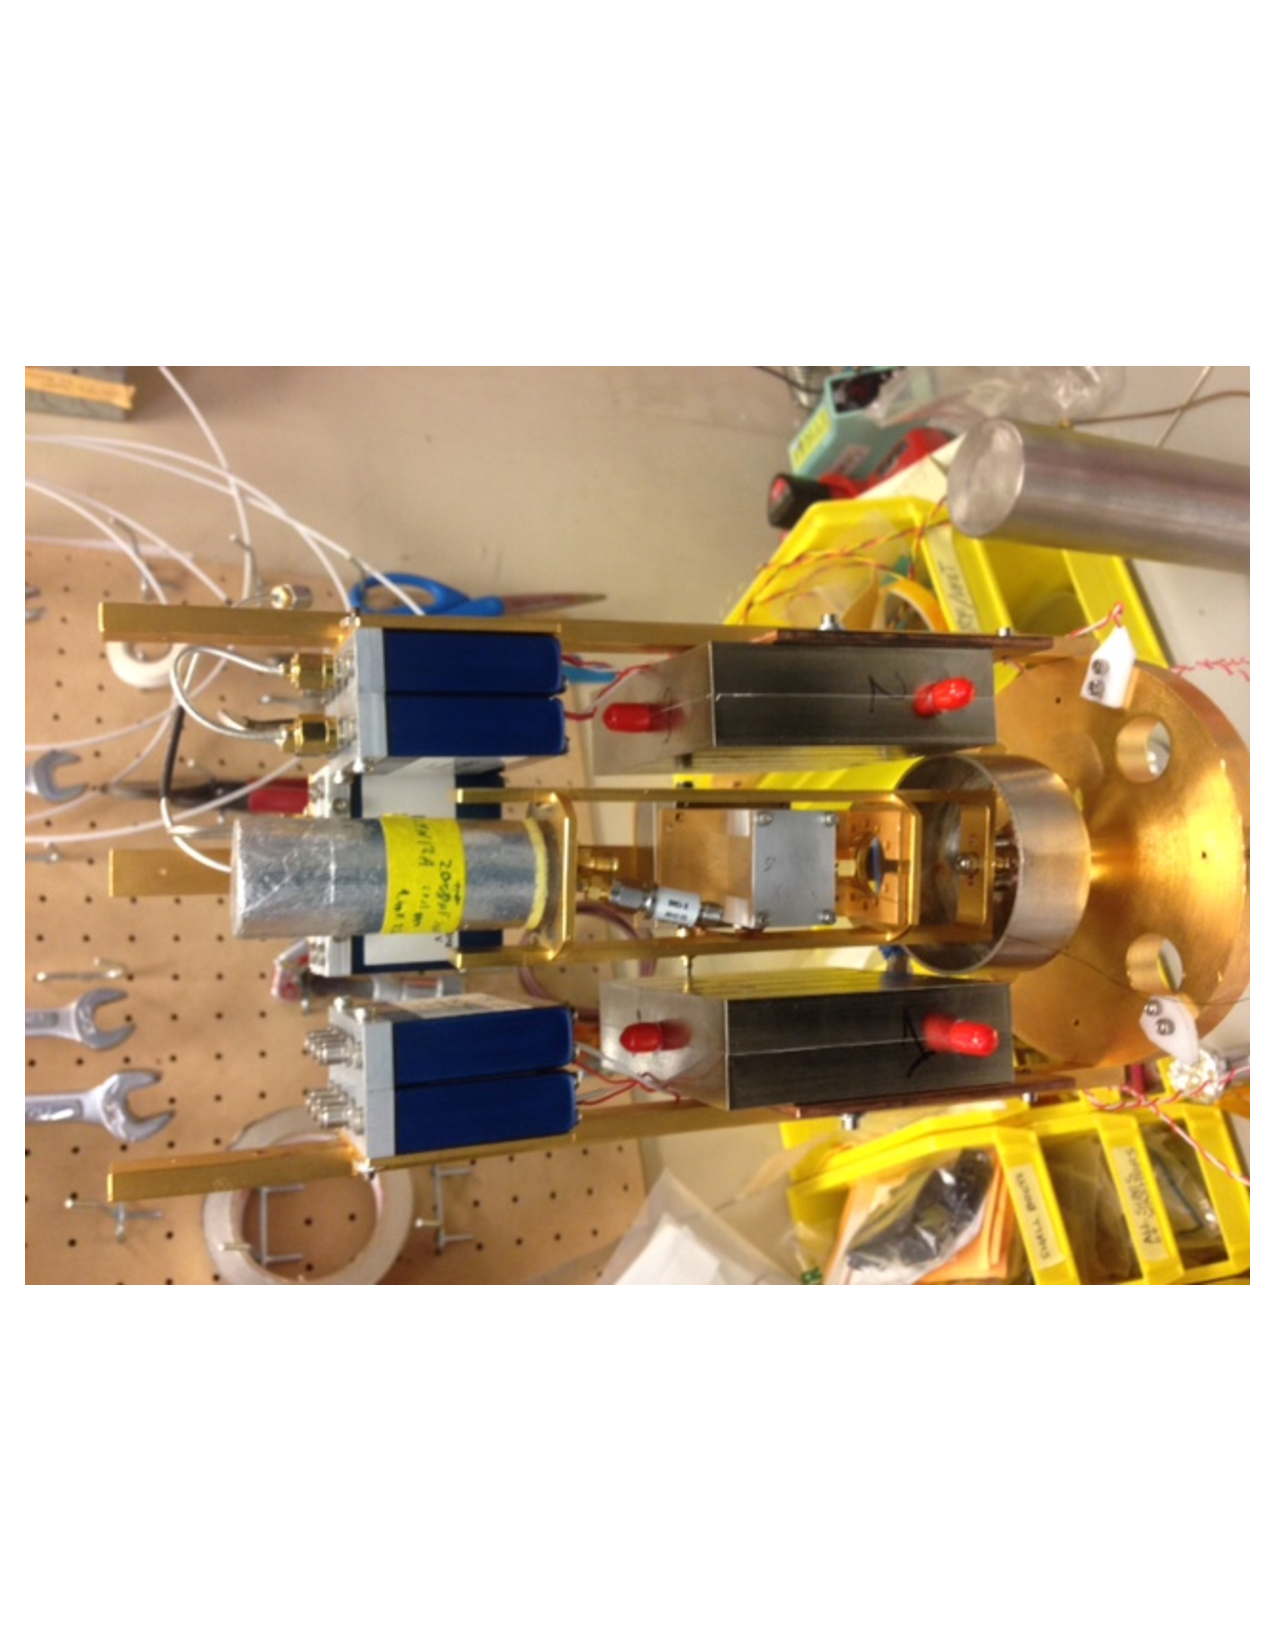
\includegraphics[width=1.1\textwidth, angle=-90]{new_squidadel}

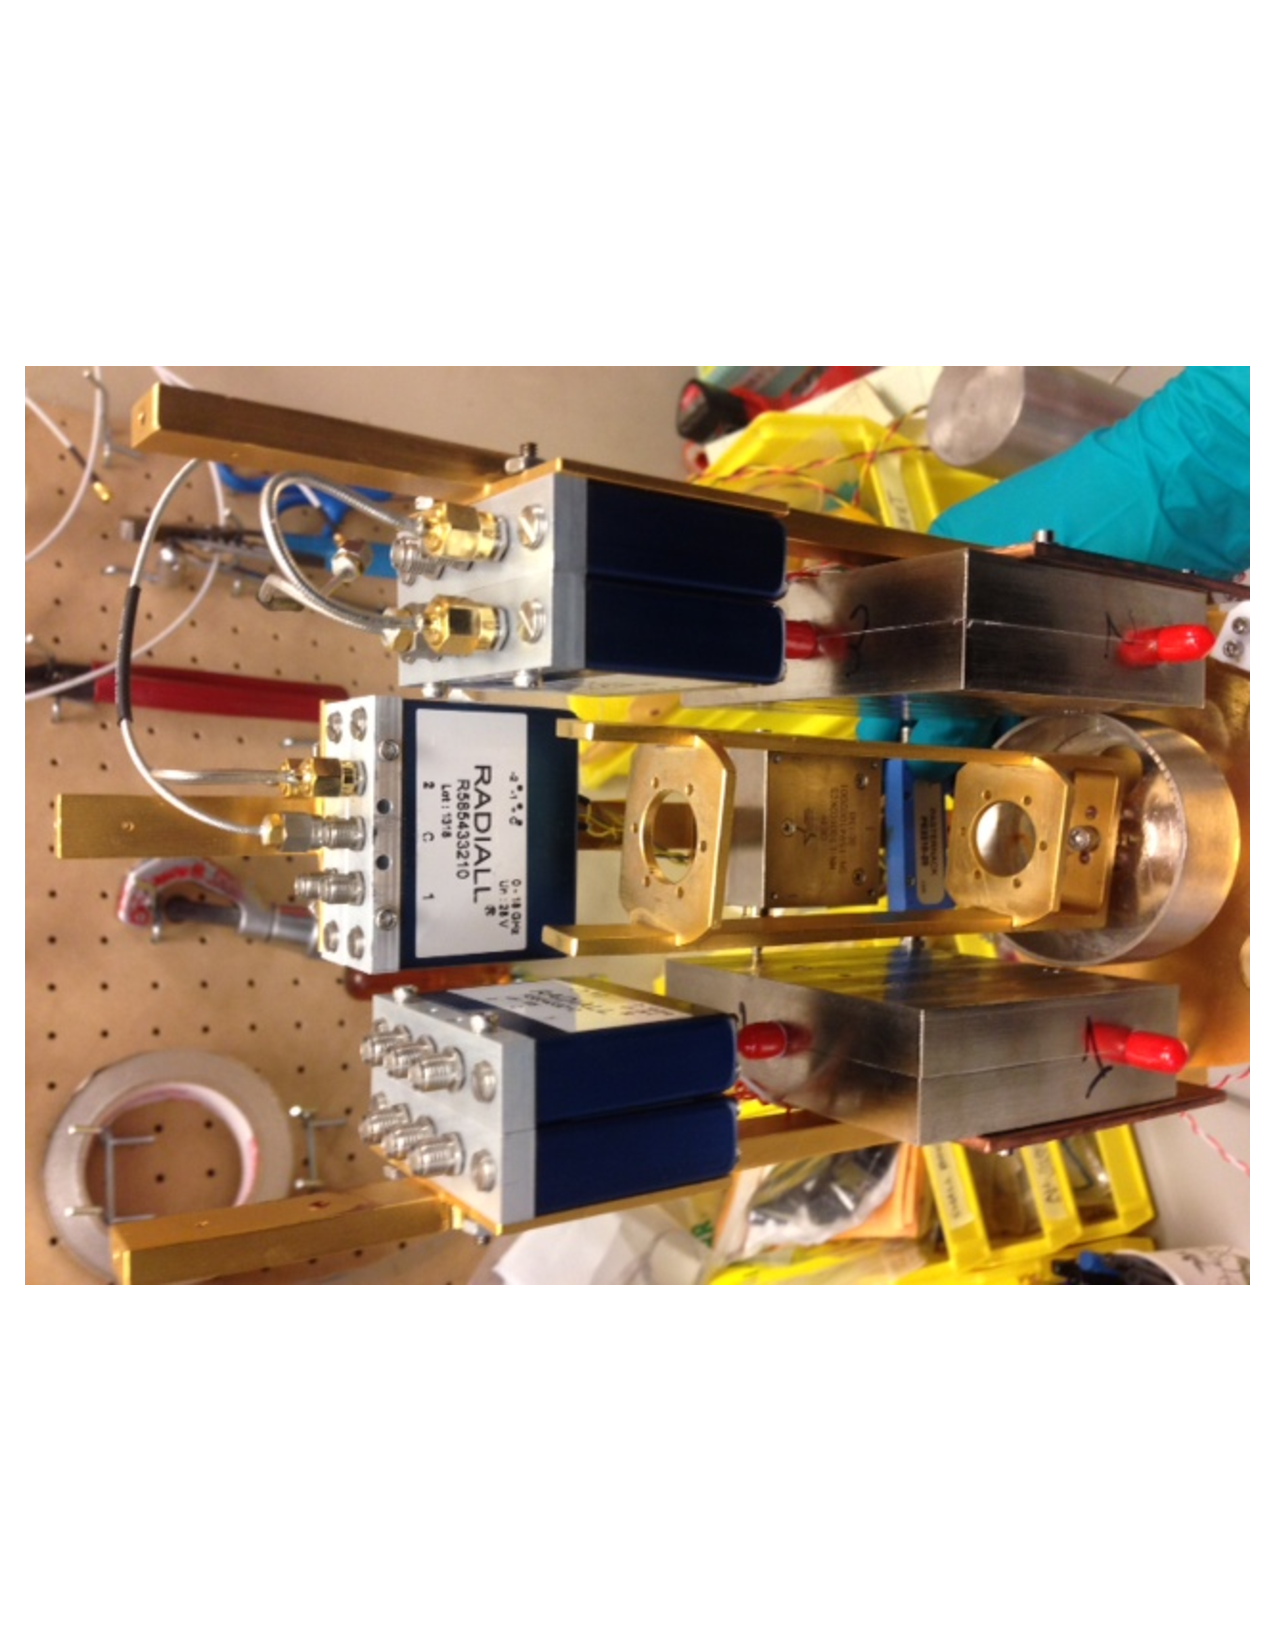
\includegraphics[width=1.1\textwidth, angle=-90]{another_view}

\end{columns}
\end{frame}

\begin{frame}
\begin{columns}
\column{0.45\textwidth}
{\color{blue} controls}
\begin{itemize}
\item[] {\tiny EPICs Driver for JPA Power Supply  [Cliff]}
\item[] {\tiny EPICs Driver for JPA Pump Tone  [Cliff]}
\item[] {\tiny Upgrade MSA Current Source [Cliff]}
\end{itemize}

{\color{blue} wiring/sensors}
\begin{itemize}
\item[] {\tiny Bundle squidadel dc wiring [Gray]}
\item[] {\tiny Set up Cable E for Sidecar piezo/temp sensor wires + JPA bias [Cliff]}
\item[] {\tiny Replace RF feedthrough 'nuzzlie' [Lisa]}
\item[] {\tiny Remake holder for noise sources  [Ana]}
\item[] {\color{red} \tiny Mount Sidecar hall probe/temp sensor}
\end{itemize}

{\color{blue} hemts}
\begin{itemize}
\item[] {\tiny Set up Sidecar HEMT [Gray]}
%\item[] {\color{red} \tiny Install Ch1 HEMTs [Ana]}
\item[]  {\color{red} \tiny  Resolder LB63 connector for bias pins}
\item[]  {\color{red} \tiny  Rebias Ch1 and Ch2 HEMTs}
\end{itemize}



\column{0.6\textwidth}
{\color{blue} cabling}
\begin{itemize}
\item[]  {\tiny RF feedthrough collar [Dima]}
\item[] {\tiny  Epoxy RF feedthroughs in anchoring rows [Kiva]}
\item[]  {\color{red} \tiny **Install Coax Co. cables**}
\item[]  {\color{red} \tiny Heat sink cables}
\item[]  {\color{red} \tiny Put in attenuators}
\item[] {\color{red} \tiny Check transmission through cable assemblies}
\end{itemize}

{\color{blue} squidadel (this iteration)}
\begin{itemize}
\item[] {\tiny Make adaptor plates to hold circulators on posts [Ana]}
\item[] {\tiny Make JPA mount [Machine Shop]}
\item[] {\tiny Add two more bolts to inner holder [Dima]}
%\item[] {\color{red} \tiny Verify Mumetal shield still functioning}
\item[] {\color{red} \tiny Remount temperature sensors and hall probe}
\end{itemize}

{\color{blue} squidadel (next iteration)}
\begin{itemize}
\item[] {\color{red} \tiny Remake posts to fit more circulators}
\item[] {\color{red} \tiny Remake holder to fit more JPAs}
\item[] {\color{red} \tiny Install superconducting RF cable}
\end{itemize}
\end{columns}
\end{frame}

\begin{frame}{Side Dewar}
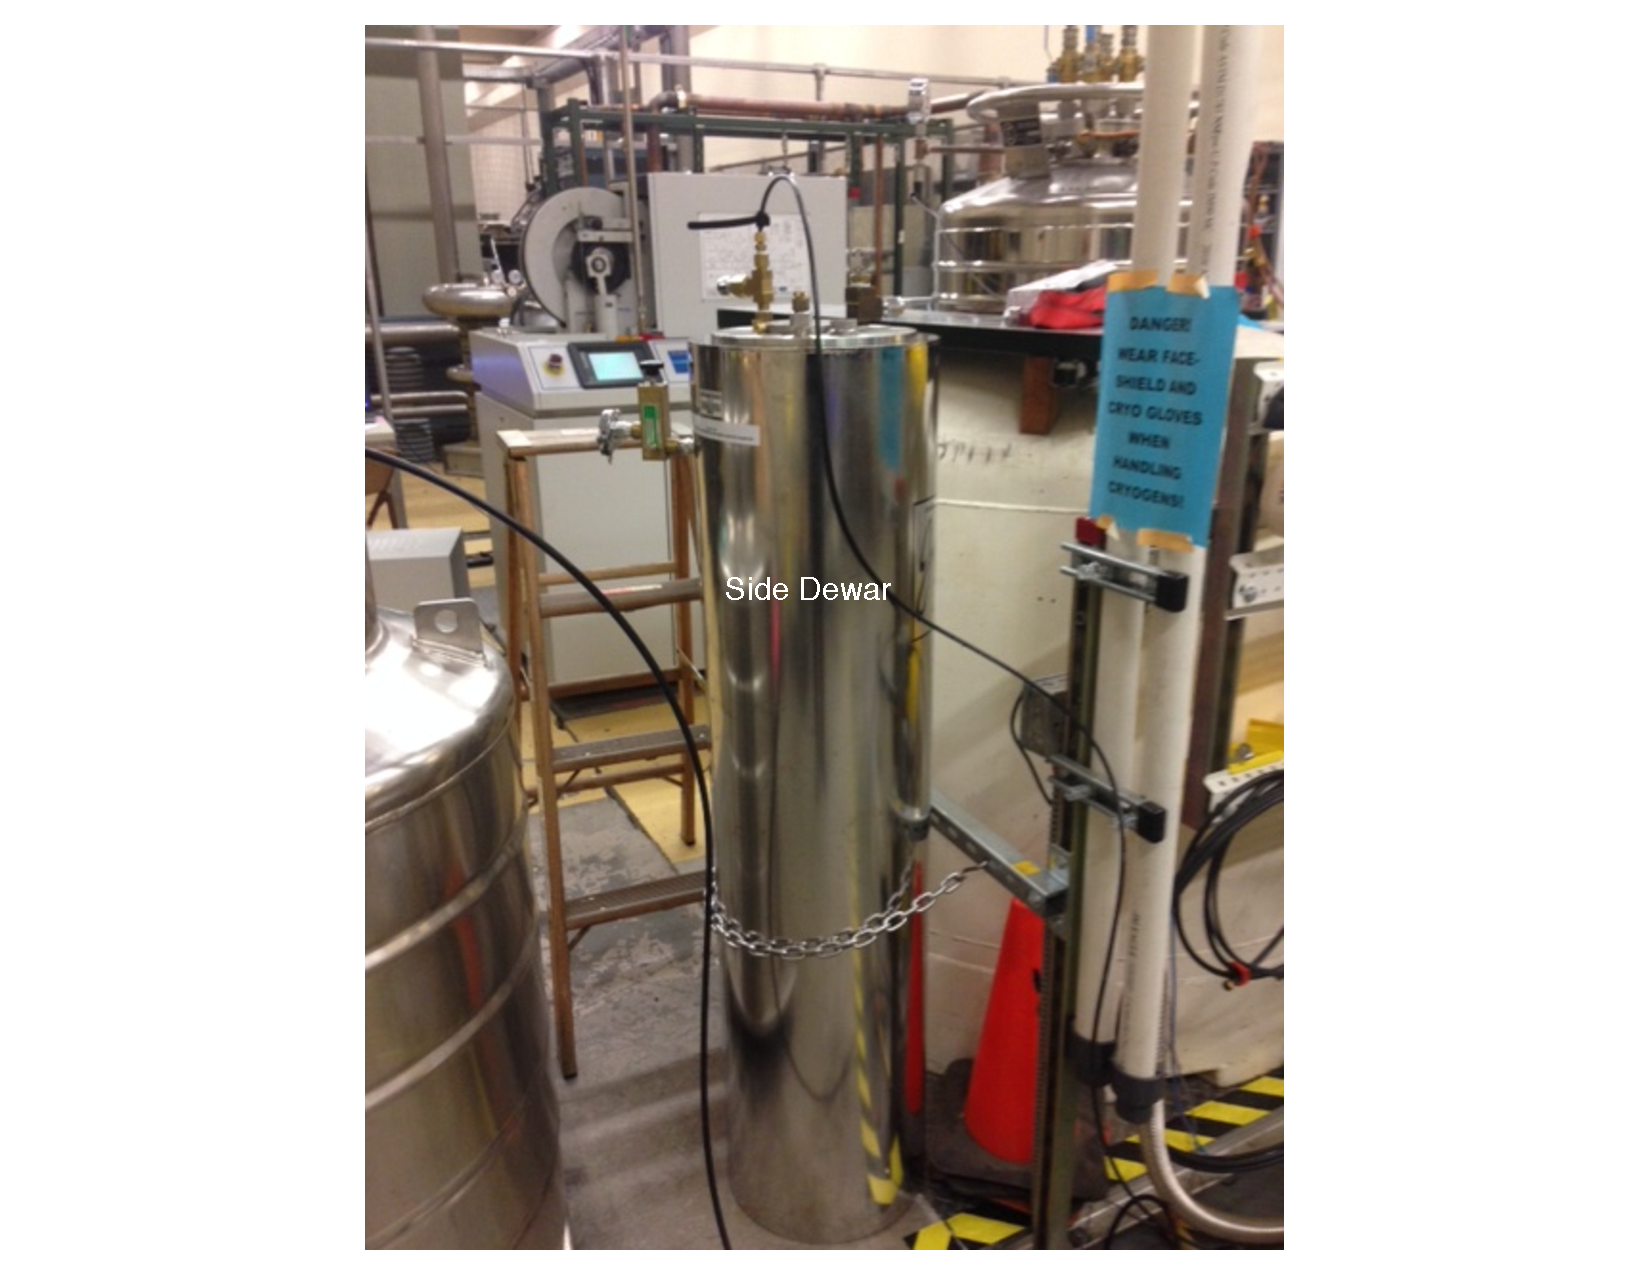
\includegraphics[width=.7\textwidth]{side_dewar}
\end{frame}

\begin{frame}{Additional}
\end{frame}

\begin{frame}{Coverage}
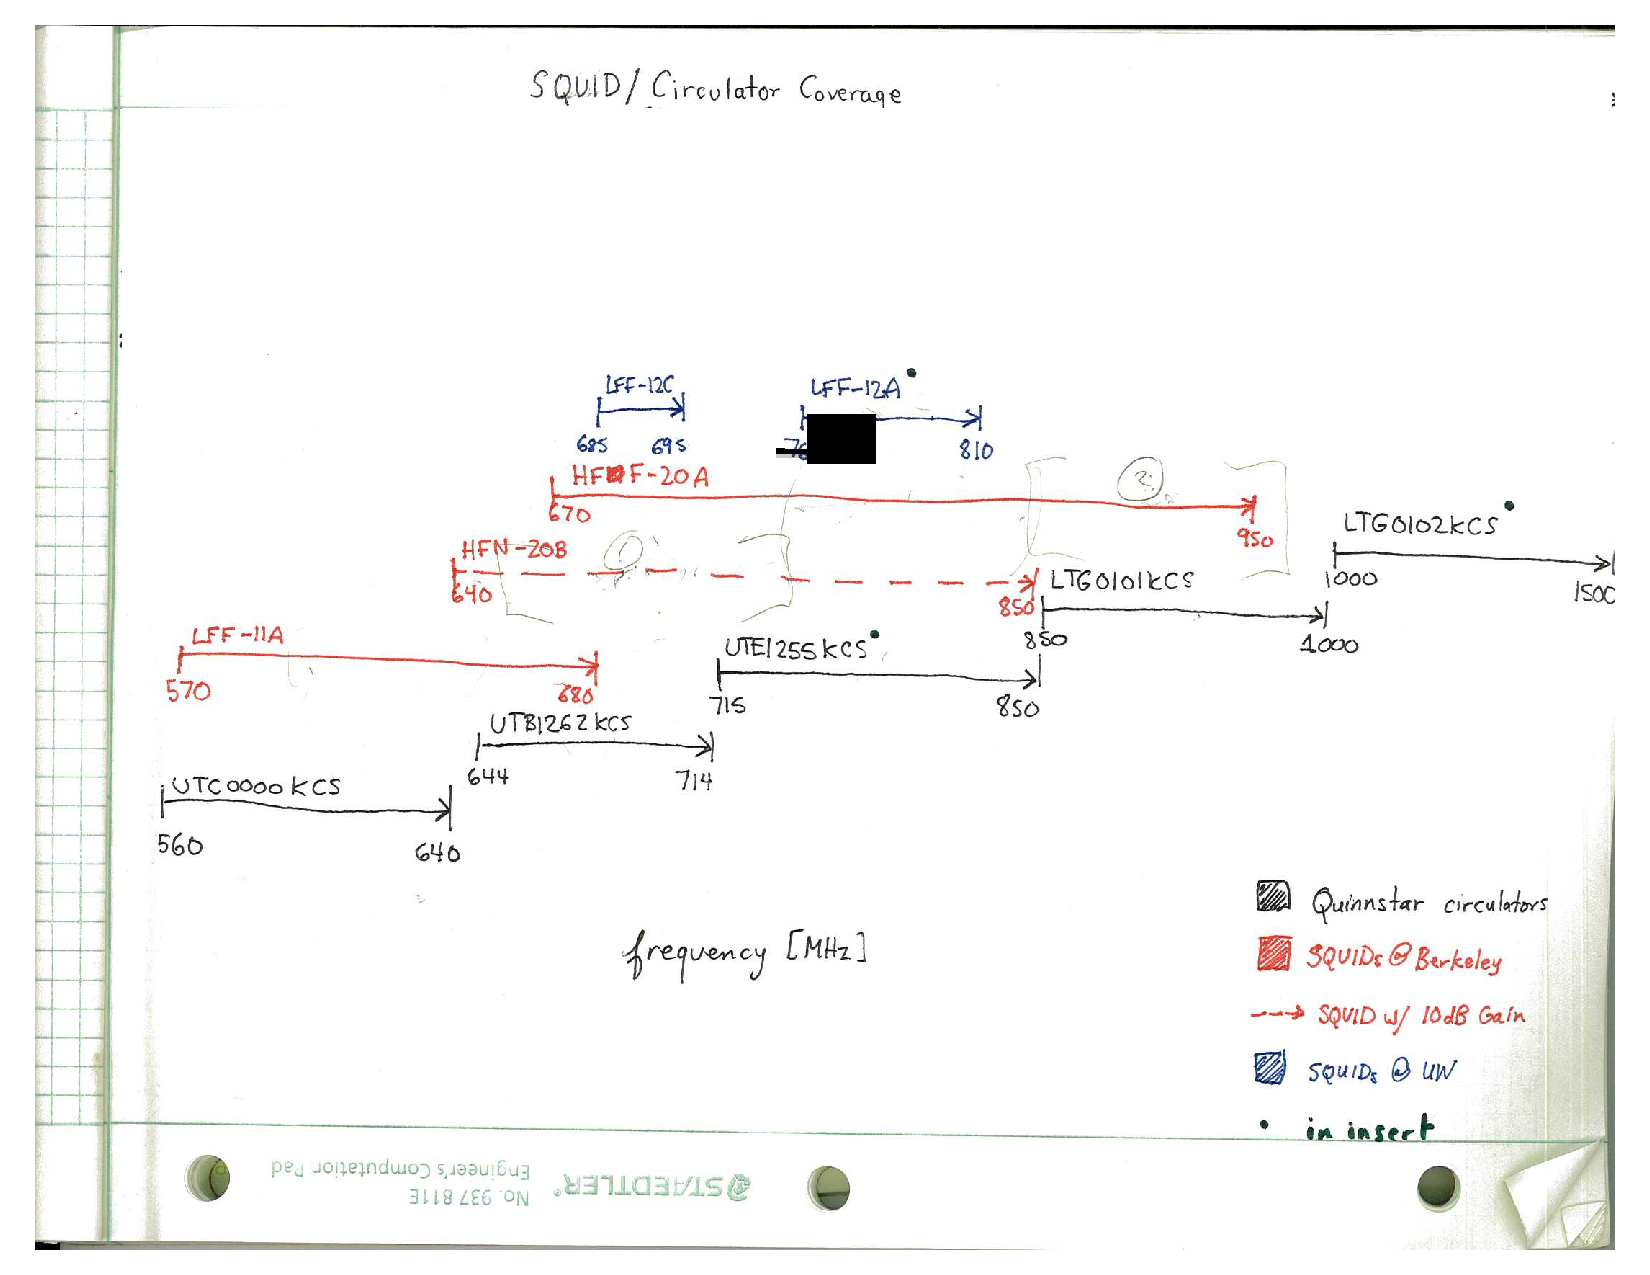
\includegraphics[width=.9\textwidth]{copier_20150502_210746_pg2_revised}
\end{frame}

\begin{frame}{Run Coverage}
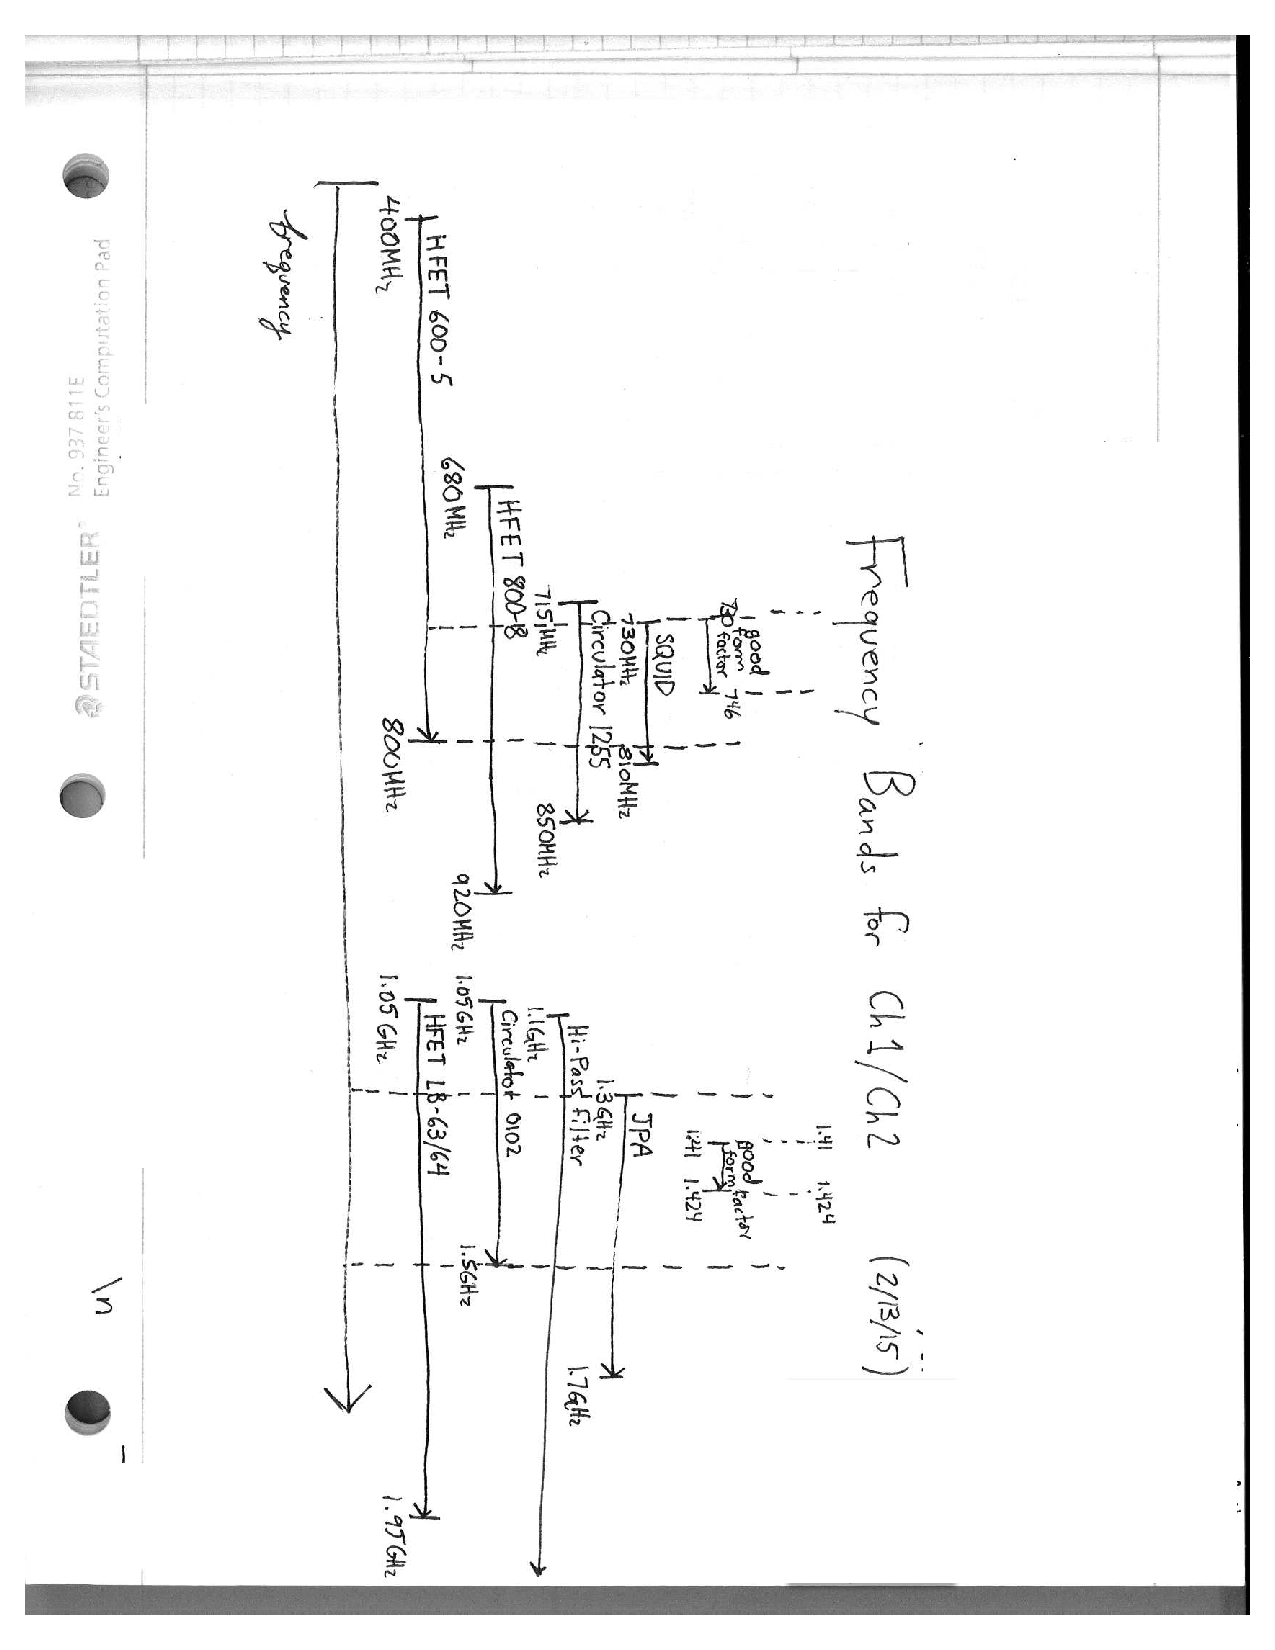
\includegraphics[width=.7\textwidth, angle=90]{copier_20150502_210746_pg1}
\end{frame}

\begin{frame}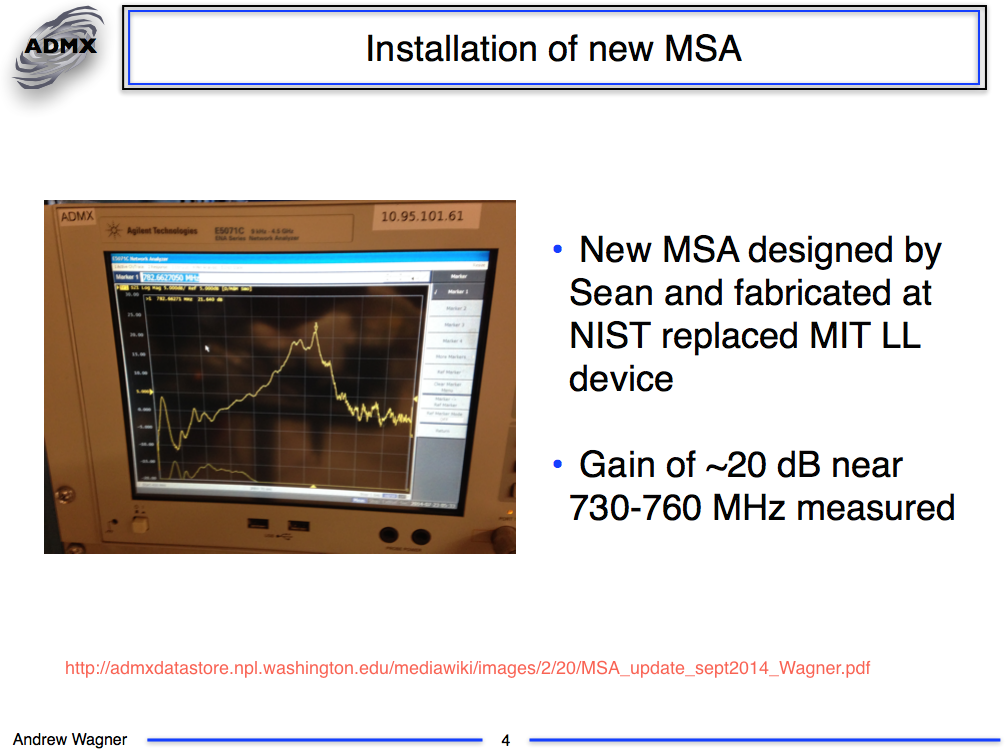
\includegraphics[width=\textwidth]{wagner_frequency}
\end{frame}

\begin{frame}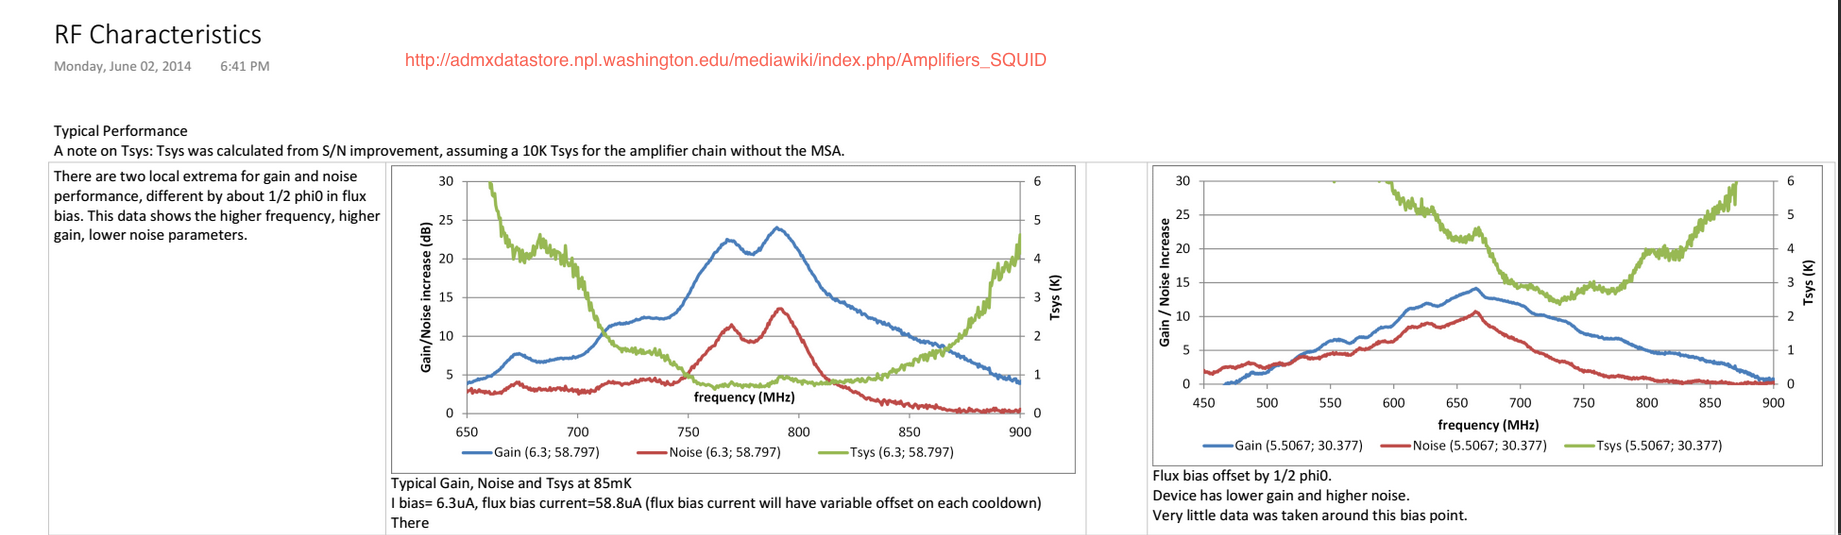
\includegraphics[width=\textwidth]{sean_frequency}
\end{frame}

\begin{frame}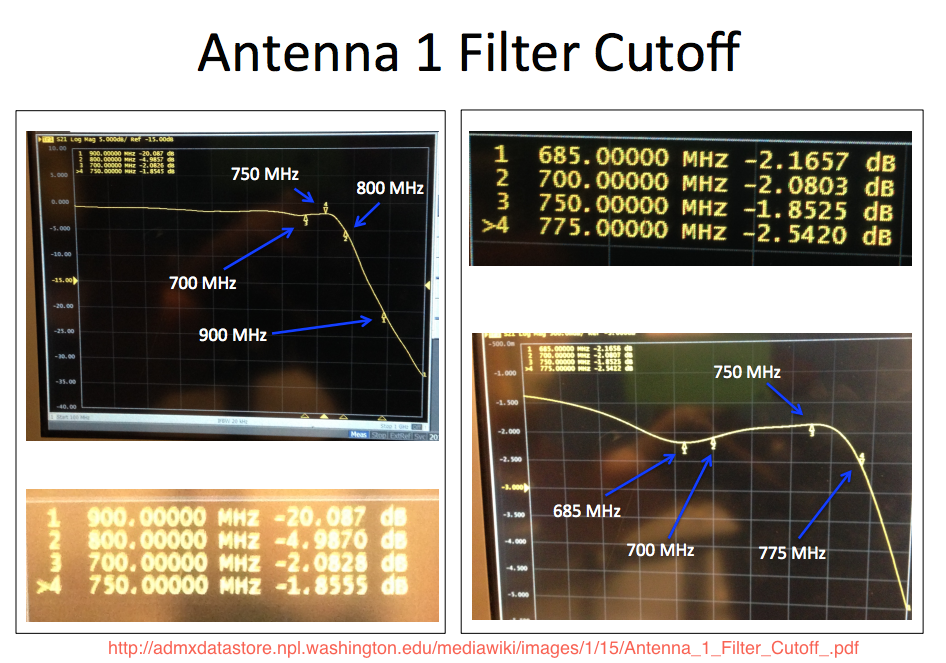
\includegraphics[width=\textwidth]{antenna_filter_cutoff}
\end{frame}

\begin{frame}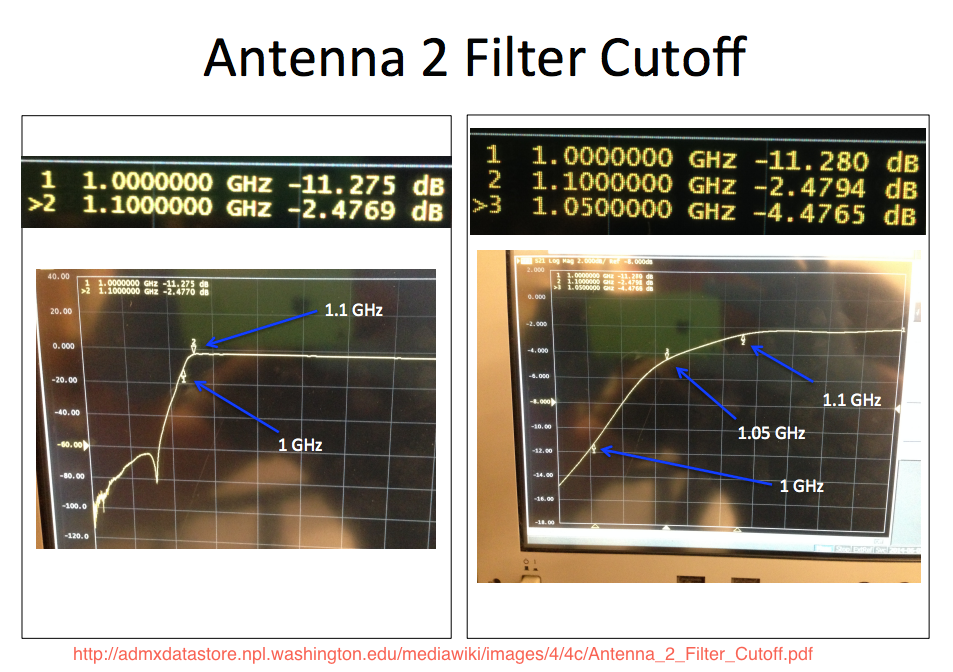
\includegraphics[width=\textwidth]{antenna_2}
\end{frame}

\end{document}
